\section{Methods}
\todo[inline]{differentiate between cycle in network and loop in flux}
\todo[inline]{mention scaling of epsilon; why eps = 1 in computation}
In \cref{section:metabolic_networks}, we have seen how mathematical optimization can be used to predict fluxes $\bold v$ in a cell that optimize a biological objective. In particular ll-FBA (\cref{problem:llfba}) can be used to predict fluxes that do not contain internal loops. However, ll-FBA is difficult to solve due to the constraint that $\Delta \mu_i$ and $v_i$ have to be of opposite sign, unless $v_i=0$, which is modeled by a disjunction. In this thesis, we compare the runtime of the big-M reformulation of ll-FBA to the convex-hull reformulation and to solving the problem by adding cutting planes. 

\todo[inline]{technical setup, github link}
The code is written in \textsf{Julia} 1.9.0. We use \textsf{JuMP} \cite{JuMP} and \textsf{MathOptInterface} \cite{mathoptinterface} to build the mathematical models. The MIP solver used in the experiments is \textsf{SCIP} \cite{SCIP}. The LP solver used is \textsf{HiGHS} \cite{HiGHS}. We use \textsf{COBREXA}\cite{cobrexa} to load the biological model data.

\todo[inline]{rewrite following section, shorten section}
\todo[inline]{present more why you have done what and then link the sections}
% delayed constrained generation for cuts
In \cref{section:feasibility_test}, we explain briefly how we test for a solution whether it does not contain internal loops. 
In \cref{section:llfba_variants}, we see how ll-FBA can be reformulated with indicator constraints, and with big-M constraints.
In \cref{section:blocking_cycles}, we take a solution to the FBA problem (\cref{problem:fba}) which may contain internal loops. Loops are identified and cuts are added to the ll-FBA formulation to exclude solutions that contain a specific loop from the feasible region.
In \cref{section:no_good_cuts}, we solve a relaxed version of ll-FBA, where we solve an FBA, but assign binary variables dependent on the directionality of $\bold v$. If a solution to the relaxed problem is not a feasible solution to the ll-FBA problem, a cut is added to the relaxed problem that cuts off the assignment of binary variables. This procedure is repeated until a solution is found that is a feasible solution to ll-FBA. 
We will see in \cref{section:cb} how to generate stronger cuts than a no-good cut using combinatorial Benders' cuts. The ll-FBA problem is split into a master problem and subproblem and we exploit the duality of the infeasible subproblem to generate cuts that include a subset of binary variables only. 
Another type of cuts are intersection cuts, explained in \cref{section:methods_interscetion_cuts}. The feasible region is split into the polyhedral set $P$, which contains the inequality and equality constraints, and the set $S$, which contains the disjunctions. An S-free set $C$ is defined around a solution $\boldsymbol{\tilde x}$ that lies in $P$ but not in $S$. The intersection cut is the hyperplane going through the intersection of the conic relaxation at $\boldsymbol{\tilde x}$ with $C$. 
In \cref{section:disjunctive_programming}, the ll-FBA problem is written as disjunctive problem, which includes a binary variable for each disjunct. The problem is then solved by using the big-M reformulation and the convex-hull reformulation. In \cref{section:models} we introduce the data that is used for the experiments.

% \todo[inline]{put FBA and ll-FBA in standard form}
% \todo[inline]{explain why indicator constraints can be used in CB}
% \todo[inline]{add pseudo code}

\subsection{Feasibility Test} \label{section:feasibility_test}
For a given flux distribution $\boldsymbol{\tilde{v}}$ and the corresponding directions $\boldsymbol{\tilde{a}}$ the following problem is feasible if it is loopless:
\begin{maxi!}
    {\scriptstyle \boldsymbol{\Delta \mu}, \boldsymbol \mu}{0}{\label[problem]{problem:feasiblityCheck}}{} 
    \addConstraint{-M \leq \Delta \mu_i \leq - \epsilon \quad} {\forall i \in \mathcal{I}: \tilde{a_i} = 1}    
    \addConstraint{\epsilon \leq \Delta \mu_i \leq M \quad} {\forall i \in \mathcal{I}: \tilde{a_i} = 0}        
    \addConstraint{\boldsymbol{\Delta \mu} = \bold S_{\mathcal{I}}^\intercal \boldsymbol \mu}{}
    % \addConstraint{\mu \in \mathbb{R}^m}
    % \addConstraint{\Delta \mu \in \mathbb{R}^n}
    % \addConstraint{v \in \mathbb{R}^n}
    % \addConstraint{S \in \mathbb{R}^{m\times n}}
\end{maxi!} 
\quad where we set the big-M constant to 1000 and $\epsilon$ to 1. 

Note that if $\tilde{v_i} = 0$, the reaction can be removed from the problem by removing the reaction from $\bold S_{\mathcal{I}}$ and without adding variable $\Delta \mu_i$. 
\cref{problem:feasiblityCheck} can also be used to test the looplessness of a solution and a subset of internal reactions by setting the flux of all other reactions to zero.

Going back to the example visualized in \cref{fig:loop} in \cref{section:fba}, for the solution $\boldsymbol{\tilde v} = (10, 30, 30, -20, 10)$ where $\tilde v_2, \tilde v_3, \tilde v_4$ are the fluxes through the internal reactions, and $\boldsymbol{\tilde a} = (1,1,0)$. The solution contains a loop and \cref{problem:feasiblityCheck} is infeasible. 

For the loopless solution $\boldsymbol{\tilde v} = (10, 10, 10, 0, 10)$, we only look at the non-zero internal fluxes $\tilde v_2, \tilde v_3$ and the corresponding directionality is $\boldsymbol{\tilde a} = (1,1)$. \cref{problem:feasiblityCheck} is feasible, and the solution is $\boldsymbol{\Delta \mu}=(-1, -1)$ and $\boldsymbol \mu = (2,1,0)$. 

\subsection{Loopless FBA Formulations} \label{section:llfba_variants}
We can reformulate \cref{problem:llfba} to no longer write the disjunctions explicitly.
The mixed-integer program of flux balance analysis without unbounded internal cycles using indicator constraints \cite{elimination_infeasible_loops}:

\begin{maxi!}
    {\scriptstyle \bold v, \bold a, \boldsymbol{\Delta \mu}, \boldsymbol \mu}{\bold c^\intercal \bold v}{\text{\textbf{ll-FBA (indicator):}} \label[problem]{problem:thermo_fba_indicator}}{}
    \addConstraint{\bold S \bold v=\bold 0} \label[constraint]{constraint:thermo_fba_indicator_b}
    \addConstraint{\bold l \leq \bold v \leq \bold u} \label[constraint]{constraint:thermo_fba_indicator_c}
    \addConstraint{a_i = 1}{\quad \implies \quad v_i \geq 0}{\quad \forall i \in \mathcal{I}} \label[constraint]{constraint:thermo_fba_indicator_d}
    \addConstraint{a_i = 1}{\quad \implies \quad \Delta \mu_i \leq - \epsilon}{\quad \forall i \in \mathcal{I}} \label[constraint]{constraint:thermo_fba_indicator_e}
    \addConstraint{a_i = 0}{\quad \implies \quad v_i \leq 0}{\quad \forall i \in \mathcal{I}} \label[constraint]{constraint:thermo_fba_indicator_f}
    \addConstraint{a_i = 0}{\quad \implies \quad \Delta \mu_i \geq \epsilon}{\quad \forall i \in \mathcal{I}} \label[constraint]{constraint:thermo_fba_indicator_g}
    % \addConstraint{\bold B^\intercal \boldsymbol{\Delta \mu} = \bold 0}
    \addConstraint{\boldsymbol{\Delta \mu} = \bold S_{\mathcal{I}}^\intercal \boldsymbol \mu} \label[constraint]{constraint:thermo_fba_indicator_h}
    % \addConstraint{a \in \{0,1\}^n}
    % \addConstraint{\Delta \mu \in \mathbb{R}^n}
    % \addConstraint{v \in \mathbb{R}^n}
    % \addConstraint{S \in \mathbb{R}^{m\times n}}
\end{maxi!}

The mixed-integer program of flux balance analysis without unbounded internal cycles using big-M constraints \cite{elimination_infeasible_loops}:
%TODO dimension of variables

\begin{maxi!}
    {\scriptstyle \bold v, \bold a, \boldsymbol{\Delta \mu}, \boldsymbol \mu}{\bold c^\intercal \bold v}{\text{\textbf{ll-FBA (big-M):}} \label[problem]{problem:thermo_fba_bigM}}{}
    \addConstraint{\bold S \bold v= \bold 0} 
    \addConstraint{l \leq v \leq u}
    \addConstraint{-Ma_i + \epsilon(1-a_i) \leq \Delta \mu_i \leq - \epsilon a_i + M(1-a_i) \quad \forall i \in \mathcal{I}}        
    \addConstraint{-M(1-a_i) \leq v_i \leq M a_i \quad \forall i \in \mathcal{I}}
    % \addConstraint{\bold B^\intercal \boldsymbol{\Delta \mu} = \bold 0} \label[constraint]{constraint:thermo_fba_bigM_f}
    \addConstraint{\boldsymbol{\Delta \mu} = \bold S_{\mathcal{I}}^\intercal \boldsymbol \mu} \label[constraint]{constraint:thermo_fba_bigM_f}
    % \addConstraint{a \in \{0,1\}^n}
    % \addConstraint{\Delta \mu \in \mathbb{R}^n}
    % \addConstraint{v \in \mathbb{R}^n}
    % \addConstraint{S \in \mathbb{R}^{m\times n}}
\end{maxi!}
The big-M formulation ensures the opposite sign of $v_i$ and $\Delta \mu_i$ if $v_i \neq 0$. If the flux through reaction $i$ is a forward flux, that is $v_i > 0$ and $a_i=1$, it holds that $-M \leq \Delta \mu_i \leq -\epsilon$ and analogously for a backward flux. We set $\epsilon$ to 1, and the big-M constant is the maximal absolute value of the flux bounds $\bold l, \bold u$. \todo[inline]{reference scaling again}
As explained in \cref{section:ll_fba}, \cref{constraint:thermo_fba_indicator_h,constraint:thermo_fba_bigM_f} can be replaced by $\bold B^\intercal \boldsymbol{\Delta \mu} = \bold 0$.

\subsection{Blocking Cycles} \label{section:blocking_cycles}
\todo[inline]{use CycleFreeFlux instead?}
\unsure[inline]{mention CycleFreeFVA here or in bio section}
We take an optimal solution  $\bold v^*$ to \cref{problem:fba}. The metabolic network and the  $\bold v^*$ are transformed such that the hyperarcs are split into simple directed edges. We search for loops in the transformed graph on edges with nonzero flux. Finally, we check whether the loop found in the transformed graph is a thermodynamically infeasible loop in the metabolic network. An internal loop can be removed by adding a constraint to \cref{problem:llfba_original}. 

The hyperarcs represented by $\bold S$ are split up by replacing each hyperarc $E= (H,T)$ by $k$ simple directed edges for every pair in $H \times T$. The transformed matrix is denoted by $\bar{\bold S}$. Assume the flux though hyperarc $E$ is $v^*_E$. $\bar{\bold v}$ has then $n$ entries with $v^*_E$.
For every nonzero reaction in $v^*$, the corresponding reactions of $\bar{\bold S}$ are used to construct a simple directed graph $G$. We use the \textsf{Graph} package to build the graph and \textsf{simplecycles\_iter} %\footnote{\url{https://juliagraphs.org/Graphs.jl/dev/algorithms/cycles/#Graphs.simplecycles_iter}} 
to compute the set of cycles in $G$ \cite{Graphs2021}. We test for a cycle in the transformed network, whether the corresponding reactions in $\bold S$ are thermodynamically feasible (see \cref{section:feasibility_test}).
To block a given cycle, a Boolean expression is added as a constraint ensuring that the $a_i$'s for reactions $i$ in the cycle are assigned differently. 

Suppose we have a solution that contains a loop $\boldsymbol \ell$ %: $\bold S_{\mathcal{I}} \boldsymbol \ell = \bold 0$, 
and let $\bold a$ be the corresponding binary variables indicating the direction of the flux. We can write the assignment of binary variables as Boolean expression: $t_1 \land ... \land t_i \land ... t_{|\mathcal{I}|}$, where $t_i = a_i$ if $a_i=1$ and otherwise $t_i = 1 -a_i$.
To block the cycle, the assignment of the $a_i$'s has to be constrained: 
    $\neg (t_1 \land ... \land t_i \land ... t_{|\mathcal{I}|}) \, = 1$.
Formulating the expression as linear constraint yields:
    $t_1 + ... + t_i + ... t_{|\mathcal{I}|} \geq 1$.
    % # to block cycle: ¬(a1 ∧ a2 ∧ a3) = ¬a1 ∨ ¬a2 ∨ ¬a3 >= 1
    % # ¬a1 = 1 - a1 => 
    % # 1-a1 ∨ 1-a2 ∨ 1-a3 >= 1 
    % # -a1 ∨ -a2 ∨ -a3 >= 1-3 = -2
    % # for backward arc: ¬(¬a1) = a1

A detected cycle can be blocked by a cut in the thermodynamic feasible FBA. The solution will not be impacted, but the run time can be affected. 
% numbers of cycles
% The number of cycles blocked has a strong impact on the run time. There is a significant slow down if the number of cycles is greater than ... 
% shortest cycles
We filter the thermodynamically infeasible cycles in the set of cycles found in the transformed graph. Instead of blocking all detected cycles, we experiment with blocking the smallest cycles, which potentially leads to stronger cuts. 

\todo[inline]{example}

\subsection{No-Good Cuts} \label{section:no_good_cuts}
When using no-good cuts to solve ll-FBA, the solving procedure is divided into first solving the relaxed problem and then checking the feasibility of the solution to the relaxed problem. 
The following relaxed version of \cref{problem:thermo_fba_indicator} is solved, where the loopless constraints are ignored, but the indicator variables $\bold a$ are assigned:
\begin{maxi!}
    {\scriptstyle \bold v, \bold a}{\bold c^\intercal \bold v}{\label[problem]{problem:noGoodCut}}{} 
    \addConstraint{\bold S \bold v= \bold 0} 
    \addConstraint{\bold l \leq \bold v \leq \bold u}
    \addConstraint{a_i = 1}{\quad \implies \quad v_i \geq 0}{\quad \forall i \in \mathcal{I}}      \addConstraint{a_i = 0}{\quad \implies \quad v_i \leq 0}{\quad \forall i \in \mathcal{I}}
\end{maxi!}

The indicator constraints can be linearized by using the big-M method.
If a solution $\bold x^{IP}$ to \cref{problem:noGoodCut} is thermodynamically infeasible, the following constraint is added:

\begin{equation} \label{noGoodCut}
\sum_{i \in \mathcal{I}: x_i^{IP}=1} a_i + \sum_{i \in \mathcal{I}: x_i^{IP}=0} (1-a_i) \leq |\mathcal{I}|-1
\end{equation}

The problem is now solved again and this procedure is repeated until a solution is thermodynamically feasible. 

As an example, let us consider the metabolic network in \cref{fig:two_internal_loops}. We have four internal metabolites $A,B,C, D$, two irreversible exchange reactions $r_1, r_5$, two irreversible internal reactions $ r_6, r_7$ and three reversible internal reactions $r_2, r_3, r_4$. We assume the following bounds on the fluxes: 
\begin{equation*} \label{Eq:bounds_loop}
    \bold l = (0,-10,-10,-20,0,0,0) \quad \bold u = (20,30,30,30,20,10,10)
\end{equation*}
\begin{figure}[h!]
    \caption{simple model with two internal loops}
    \centering
    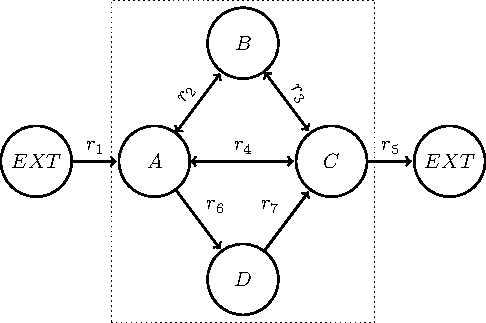
\includegraphics[width=0.8\textwidth]{Images/tikz_graphs_two_loops.pdf}
    \label{fig:two_internal_loops}
\end{figure}
\todo[inline]{show flux in color}
If we maximize the flux through the all reactions, that is $\bold c = \bold 1$, the optimal solution is $\bold v^* = (20, 30, 30, -20, 20, 10, 10)$ and $\bold a = (1,1,0,1,1)$. The solution is not thermodynamically feasible as it contains two internal loops. The corresponding no-good cut is:
\begin{equation*}
    (1-a_3) + \sum_{i \in \{1,2,4,5\}} a_i \leq 5-1
\end{equation*}

\subsection{Combinatorial Benders' Cuts} \label{section:cb}
 When deriving combinatorial Benders' cuts for ll-FBA, the solving procedure is divided into first solving the relaxed problem and then checking the feasibility of the solution to the relaxed problem, similar to the no-good cut derivation. However, instead of forbidding the infeasible solution found to the relaxed problem, we aim at identifying the variables that lead to the thermodynamic infeasibility, and potentially derive stronger cuts.

ll-FBA matches the required problem form \cref{problem:mathematical_program_CB}. We have a linear objective $\bold c^\intercal \bold v$, continuous variables $\bold v$ and $\boldsymbol{\Delta \mu}$, and a set of binary variables $\bold a$. There are linear constraints on the continuous variables \cref{constraint:thermo_fba_indicator_b,constraint:thermo_fba_indicator_c,constraint:thermo_fba_indicator_h}, and no constraints on the binary variables. The continuous variables and the binary variables are only connected by the indicator constraints (\cref{constraint:thermo_fba_indicator_d,constraint:thermo_fba_indicator_e,constraint:thermo_fba_indicator_f,constraint:thermo_fba_indicator_g}), and we can split the MIP into a master and a subproblem.
The master problem (MP) is
% \begin{maxi!}
%     {\scriptstyle \bold v, \bold a}{\bold c^\intercal \bold v}{\label[problem]{problem:masterProblem}}{} 
%     \addConstraint{\bold S \bold v = \bold 0} 
%     \addConstraint{\bold l \leq \bold v \leq \bold u}
%     \addConstraint{a_i = 1}{\quad \implies \quad v_i \geq 0}{\quad \forall i \in \mathcal{I}}      \addConstraint{a_i = 0}{\quad \implies \quad v_i \leq 0}{\quad \forall i \in \mathcal{I}}
% \end{maxi!}
\cref{problem:noGoodCut}
and the subproblem (SP) is the following \textit{parameterised program}:
\begin{maxi!}
    {\scriptstyle \boldsymbol{\mu, \Delta \mu}}{0}{\label[problem]{problem:methods_subProblem}}{} 
    \addConstraint{a_i^{MP} = 1}{\quad \implies \quad \Delta \mu_i \leq - \epsilon}{\quad \forall i \in \mathcal{I}}
    \addConstraint{a_i^{MP} = 0}{\quad \implies \quad \Delta \mu_i \geq \epsilon}{\quad \forall i \in \mathcal{I}} \label[constraint]{constraint:subProblem_c}
    % \addConstraint{c^\intercal v \geq \mathcal{UB} + \epsilon}
    \addConstraint{\boldsymbol{\Delta \mu} = \bold S_{\mathcal{I}}^\intercal \boldsymbol \mu} \label[constraint]{constraint:subProblem_d}
\end{maxi!}

\quad where $\bold a^{MP}$ are the values of a solution to the master problem. If the subproblem is infeasible, we compute a corresponding minimal infeasible subsystem (MIS) $\mathcal{C}$. The minimal infeasible subsystem contains a minimal number of constraint indices that make the subproblem infeasible.
The following combinatorial Benders' (CB) cut is added to the master problem if the subproblem is infeasible:
\begin{equation*}
\sum_{i \in \mathcal{C}: a_i^{MP}=0} a_i + \sum_{i \in \mathcal{C}: a_i^{MP}=1} (1-a_i) \geq 1
\end{equation*}
Note that if $\mathcal{C}$ contains all internal reactions $\mathcal{I}$, the CB cut corresponds to a no-good cut (\cref{noGoodCut}).

The pseudocode for the combinatorial Benders' cut procedure is shown in \cref{alg:CB}. In \textsf{build\_master\_problem}, the MP is built, which is the FBA problem with binary variables $\bold a$ that are linked to the directionality of $\bold v$. The relation between the flux variables $\bold v$ and the binary variables $\bold a$ can be expressed by indicator constraints as in \cref{problem:noGoodCut}, by big-M constraints, or by indicator constraints and big-M constraints simultaneously. The big-M constant corresponds to the maximal absolute value of lower bounds $\bold l$ and upper bounds $\bold u$.
The set of minimal infeasible subsystems is computed in \textsf{compute\_mis}, which identifies at most $m$ subsystems. The MIS search is explained in detail in \cref{section:methods_mis}. The dual problem of the infeasible subproblem is built with the \textsf{Dualization} package \cite{dualization}.
If we find a minimal infeasible subset $\mathcal{C}$, a combinatorial Benders' cut is added to the master problem. If there exists no MIS, the subproblem is feasible and thus the solution to the master problem is thermodynamically feasible. 
This process is repeated until a solution is found, that is feasible in the master problem and the subproblem and therefore also for \cref{problem:thermo_fba_indicator}. In \textsf{build\_sub\_problem}, the subproblem is built based on the thermodynamically feasible solution of the master problem to obtain the corresponding values for $\boldsymbol{\Delta \mu}$ and $\boldsymbol \mu$. 
%\unsure[inline]{shape of subproblem if there exist multiple MISs => all constraints on delta mu are added at once}

\begin{algorithm}
    \caption{ll-FBA with combinatorial Benders' cuts}\label{alg:CB}
    \begin{algorithmic}[1]
        \Require stoichiometric matrix $\bold S$, lower bound on fluxes $\bold l$, upper bound on fluxes $\bold u$, allowed number of cuts per iteration $m$, indices of internal reactions $\mathcal{I}$
        \State MP $\gets \textsf{build\_master\_problem}(\bold S, \bold l, \bold u, \mathcal{I})$
        \State $\bold{v, a} \gets \textsf{optimize(MP)}$ 
        \State $\mathcal{C} \gets \textsf{compute\_mis}(\bold S_\mathcal{I}, \bold a, m)$ \Comment{set of minimal infeasible subsystems}
        %\State $\text{SP} \gets \text{build\_sub\_problem}(\bold S_\mathcal{I},  \mathcal{C}, \bold a)$
        %\State $\text{optimize(SP)}$ 
        %\While{$\text{status(SP)} = \text{INFEASIBLE}$}
        \While{$\mathcal{C} \neq \emptyset$}
            \State $\textsf{add\_cut}(\text{MP}, \bold a, \mathcal{C})$ \Comment{combinatorial Benders' cut}
            \State $\bold v, \bold a \gets \textsf{optimize}$(MP)
            \State $\mathcal{C} \gets \textsf{compute\_mis}(\bold S_\mathcal{I}, \bold a, m)$
            % \If{ $\mathcal{C} = \emptyset$}
            %     \State $\text{status(SP)} \gets \text{OPTIMAL}$
            % \Else
            %     \State $\text{SP} \gets \text{build\_sub\_problem}(\bold S_\mathcal{I}, \mathcal{C}, \bold a)$
            %     \State $\text{optimize(SP)}$ 
            % \EndIf
        \EndWhile
        \State $\text{SP} \gets \textsf{build\_sub\_problem}(\bold S_\mathcal{I}, \mathcal{I}, \bold a)$
        \State $\boldsymbol{\Delta \mu}, \boldsymbol \mu \gets \textsf{optimize}$(SP)
    \State \Return $(\bold v, \bold a, \boldsymbol{\Delta \mu}, \boldsymbol \mu)$ \Comment{loopless flux distribution}
    \end{algorithmic}
\end{algorithm}

Going back to the metabolic network in \cref{fig:two_internal_loops}
with the objective function $f = \text{max} \, \bold 1^\intercal \bold v$, the optimal solution of the master problem is $\bold v^* = (20, 30, 30, -20, 20, 10, 10)$ and $\bold a = (1,1,0,1,1)$. 
The solution is not thermodynamically feasible, and a minimal infeasible subset is $\mathcal{C} = \{3, 4, 5\}$, which corresponds to the cycle $r_4=-10, r_6=10, r_7=10$. 
The corresponding combinatorial Benders' cut is:
\begin{equation*}
    a_3 + 1 - a_4 + 1 - a_5 \geq 1
\end{equation*}

\subsubsection*{MIS Search} \label{section:methods_mis} 
\addcontentsline{toc}{subsubsection}{\protect\numberline{}Minimal Infeasible Subset} 
If a solution to the master problem is not loopless, the subproblem is infeasible.
% To find minimal infeasible subsets, the following primal linear program of an infeasible solution \cref{Eq:subProblem} is formulated: 
% \begin{maxi!}
%     {\scriptstyle \mu}{0}{\label[problem]{problem:MISPrimal}}{} 
%     \addConstraint{\tilde{a_i} = 1}{\quad \implies \quad (S_{\mathcal{I}}^\intercal \mu)_i < 0}{\quad \forall i \in \mathcal{I}}
%     \addConstraint{\tilde a_i = 0}{\quad \implies \quad (S_{\mathcal{I}}^\intercal \mu)_i > 0}{\quad \forall i \in \mathcal{I}}
% \end{maxi!}
We use the infeasible subproblem and its corresponding dual problem to generate a minimal infeasible subsystem. 

First, the primal problem (\cref{problem:methods_subProblem}) is rewritten in inequality form.
To have the decision variable $\boldsymbol \mu$ on the left-hand side of $\leq$, the \cref{constraint:subProblem_c} is multiplied by -1:
\begin{equation*}
    \Delta \mu_i \geq \epsilon \implies - \Delta \mu_i \leq -\epsilon
\end{equation*}

We aslo subsitute $\boldsymbol{\Delta \mu}$ with $\bold S_{\mathcal{I}}^\intercal \boldsymbol \mu$
% We also capture the equality in \cref{constraint:subProblem_d} with two inequalities:
% \begin{align*}
%     \boldsymbol{\Delta \mu}^\intercal - \boldsymbol \mu^\intercal \bold S_{\mathcal{I}} &\leq \bold 0 \\
%     -\boldsymbol{\Delta \mu}^\intercal + \boldsymbol \mu^\intercal \bold S_{\mathcal{I}} &\leq \bold 0
% \end{align*}
and obtain:
\begin{maxi!}
    {\scriptstyle \bold x}{0}{\label[problem]{problem:MISPrimalStandard}}{} 
    \addConstraint{\boldsymbol{\tilde{A}} \boldsymbol \mu \leq \boldsymbol{\tilde{b}}}
\end{maxi!}
\quad where %$\bold x = (\boldsymbol{\Delta \mu}, \boldsymbol{\mu})$ and

% $\tilde{b} = -\epsilon^{|\mathcal{I}|}$ and row $i$ of $\tilde{A}$ is the row of $-(S_{\mathcal{I}}^\intercal)$ if $\tilde{a_i} = 1$ and of $(S_{\mathcal{I}}^\intercal)$ if $\tilde{a_i} = 0$. 
\begin{equation*}
    \boldsymbol{\tilde{A}} = 
    \left[\begin{aligned}
        & [\bold S_{\mathcal{I}}]_{*,i} \quad &\forall i \in \mathcal{I}: a_i^{MP} = 1\\
        - & [\bold S_{\mathcal{I}}]_{*,i} \quad &\forall i \in \mathcal{I}: a_i^{MP} = 0\\
        % &\boldsymbol{\Delta \mu}^\intercal - \boldsymbol{\mu}^\intercal \bold S_{\mathcal{I}}\\
        % -&\boldsymbol{\Delta \mu}^\intercal + \boldsymbol \mu^\intercal \bold S_{\mathcal{I}}\\
    \end{aligned}\right]  
    \quad \boldsymbol{\tilde{b}} = \left[\begin{aligned}
        -&\epsilon^{|\mathcal{C}|} \\
    \end{aligned}\right]
\end{equation*} 

% The Lagrangian of \cref{Eq:MISPrimal} is thus: 
% \begin{equation*}
%     \mathcal{L} (\mu, \lambda) = 0 + \lambda^\intercal (\tilde{A} \mu - \tilde{b})
% \end{equation*}
% where $\lambda \geq 0$ the Lagrange multiplier for the inequality constraints. 

% \begin{align*}
%     \max_{\mu} \quad \mathcal{L}(\mu, \lambda) & = \max \quad \lambda^\intercal (\tilde{A} \mu - \tilde{b}) &\\
%     & = \max \quad \lambda^\intercal \tilde{A} \mu - \lambda^\intercal \tilde{b} &\\
%     & = \max \quad \mu^\intercal (\tilde{A}^\intercal \lambda) - \tilde{b}^\intercal \lambda &\\
%     & = \{
%     \begin{array}{lr}
%         - \tilde{b}^\intercal \lambda &\text{if} \quad \tilde{A}^\intercal \lambda = 0,\\
%         \infty &\text{otherwise}
%     \end{array}
% \end{align*}

% \cite{boyd_stephen_convex_2004} \cite{aps_mosek_nodate} \cite{bishop_pattern_2006}

% The dual problem corresponding to \cref{problem:MISPrimalStandard} is then: 
% \begin{mini!}
%     {\scriptstyle \boldsymbol \lambda}{\boldsymbol{\tilde{b}^\intercal \lambda}}{\label[problem]{problem:ISDual}}{} 
%     \addConstraint{\boldsymbol{\tilde{A}}^\intercal \boldsymbol \lambda = \bold 0}{}{}
%     \addConstraint{\boldsymbol \lambda \geq \bold 0}
% \end{mini!}

We compute minimal infeasible subsystems by modifying the dual problem as explained in \cref{section:optimization_CB} (see \cref{problem:mis_lp}). 
The objective function of the dual is moved to the constraint $-\tilde{b}^\intercal \lambda = -1$, and we minimize $\sum_i w_i \lambda_i$. By modifying $\bold w$, we potentially derive several minimal infeasible subsystems to one infeasible solution. Each solution corresponds to a minimal infeasible subsystem. The nonzero elements in $\lambda$ correspond to a MIS with the set of reaction indices $\mathcal{C}$. We choose how many cuts $k$ can be added per iteration relative to the model size. For any $i \in \{1,...,k\}$, we set the $i$-th coefficient in the objective function to zero and set all other coefficients to 1. At the end of the MIS search, we filter the minimal infeasible subsystems found to have unique subsystems within each iteration.

\unsure[inline]{should we not minimise over the number of nonzero lambdas?}
% \unsure[inline]{What do MIS mean? reactions in cycle? Present minimal example}

\subsection{Intersection Cuts} \label{section:methods_interscetion_cuts}
\todo[inline]{reference optimization section more}
In order to apply intersection cuts to the loopless FBA problem \cref{problem:llfba}, the problem has to be brought in the required form:
\begin{maxi*}
    {\scriptstyle \bold x}{\bold c^\intercal \bold x}{\label[problem]{problem:mathematical_program_S_P_2}}{} 
    \addConstraint{\bold x \in S \cap P}
\end{maxi*}
We define $\bold x = (\bold v, \boldsymbol{\Delta \mu}, \boldsymbol\mu)$, where $\bold v \in \mathbb{R}^n$, $\boldsymbol{\Delta \mu} \in \mathbb{R}^{\dim (\mathcal{I})}$ and $\boldsymbol \mu \in \mathbb{R}^m$. The vector $\bold c \in \mathbb{R}^n$ has the same coefficients as the objective function in FBA \cref{problem:fba} and a coefficient of $0$ for the variables $\boldsymbol{\Delta \mu}, \boldsymbol \mu$. The polyhedral set $P$ contains solutions that respect the steady-state constraints, the bound constraints on $\bold v$ and \cref{constraint:llfba_e}:
\begin{equation*}
    \centering
    P = \{(\bold v, \boldsymbol{\Delta \mu}, \boldsymbol\mu) \, | \, \bold S \bold v= \bold 0, \, \bold l \leq \bold v \leq \bold u, \, \boldsymbol{\Delta \mu}^\intercal = \boldsymbol \mu^\intercal \bold S_{\mathcal{I}}\}
\end{equation*}

\cref{constraint:llfba_d} is captured in the set $S$ by using the same approximation as in \cref{problem:thermo_fba_indicator} and \cref{problem:thermo_fba_bigM}:
for any internal reaction $i$ the flux through the reaction $v_i$ and $\Delta \mu_i$ are of opposite sign unless $v_i=0$ in which case $\Delta \mu_i$ can be positive or negative but cannot be in the interval $(- \epsilon, \epsilon)$. $S$ is closed as it is defined using inclusive inequalities, and therefore it contains its limit points. 
\begin{align*}
    \centering
    %S &= \{(v_i, \Delta\mu_i) \, | \, \Delta \mu_i v_i < 0 \lor v_i = 0 \quad \forall i \in \mathcal{I}\} \\
    S &= \{(v_i, \Delta\mu_i) \, | \, (v_i \geq 0, \, \Delta \mu_i \leq - \epsilon) \lor (v_i \leq 0, \, \Delta \mu_i \geq \epsilon) \quad \forall i \in \mathcal{I}\}
\end{align*}
The intersection of $P$ and $S$ is the feasible region of the ll-FBA problem. 
\todo[inline]{define A, b (to understand what $\tilde A$) means later}

As explained in \cref{section:optimization_intersection_cuts}, in order to get an intersection cut we require an $S$-free set $C$ containing the relaxed solution $\boldsymbol{\tilde x}$. Let $\boldsymbol{\tilde x} = (\boldsymbol{\tilde v}, \boldsymbol{\tilde{\Delta \mu}}, \boldsymbol{\tilde \mu})$ be an optimal solution to the relaxed LP which is in $P$ but not in $S$. There must be at least one reaction $i$ for which holds $\Delta \mu_i v_i > 0$ \todo[inline]{include interval -1, 1}. One of the maximal $S$-free sets below contains such an optimal solution:
\begin{align*}
    C_1 &= \{(v_i, \Delta\mu_i) \, | \, \Delta \mu_i \geq - \epsilon, \, v_i \geq 0\} \\
    C_2 &= \{(v_i, \Delta\mu_i) \, | \, \Delta \mu_i \leq \epsilon, \, v_i \leq 0\} %\\
    % C_3 &= \{(v_i, \Delta\mu_i) \, | \, -1 \leq \Delta \mu_i \leq 1 \, v_i \in \mathcal{I} \}
\end{align*}
% \unsure[inline]{add two more plots for other S-free sets}
% \todo[inline]{add $C_3$? can be tilted}
Suppose that $\tilde v_i > 0$ and $\tilde{\Delta \mu_i} > -\epsilon$. Such a solution is not in $S$ but contained in $C_1$ \todo[inline]{projected into space of $(v_i \Delta \mu_i)$}. A diagram for this case is shown in \cref{fig:intersection_cut}. If $\tilde v_i < 0$ and $\tilde{\Delta \mu_i} < \epsilon$ the solution is contained in $C_2$.

\begin{figure}[h!]
    \caption{diagram of an intersection cut for ll-FBA}
    \centering
    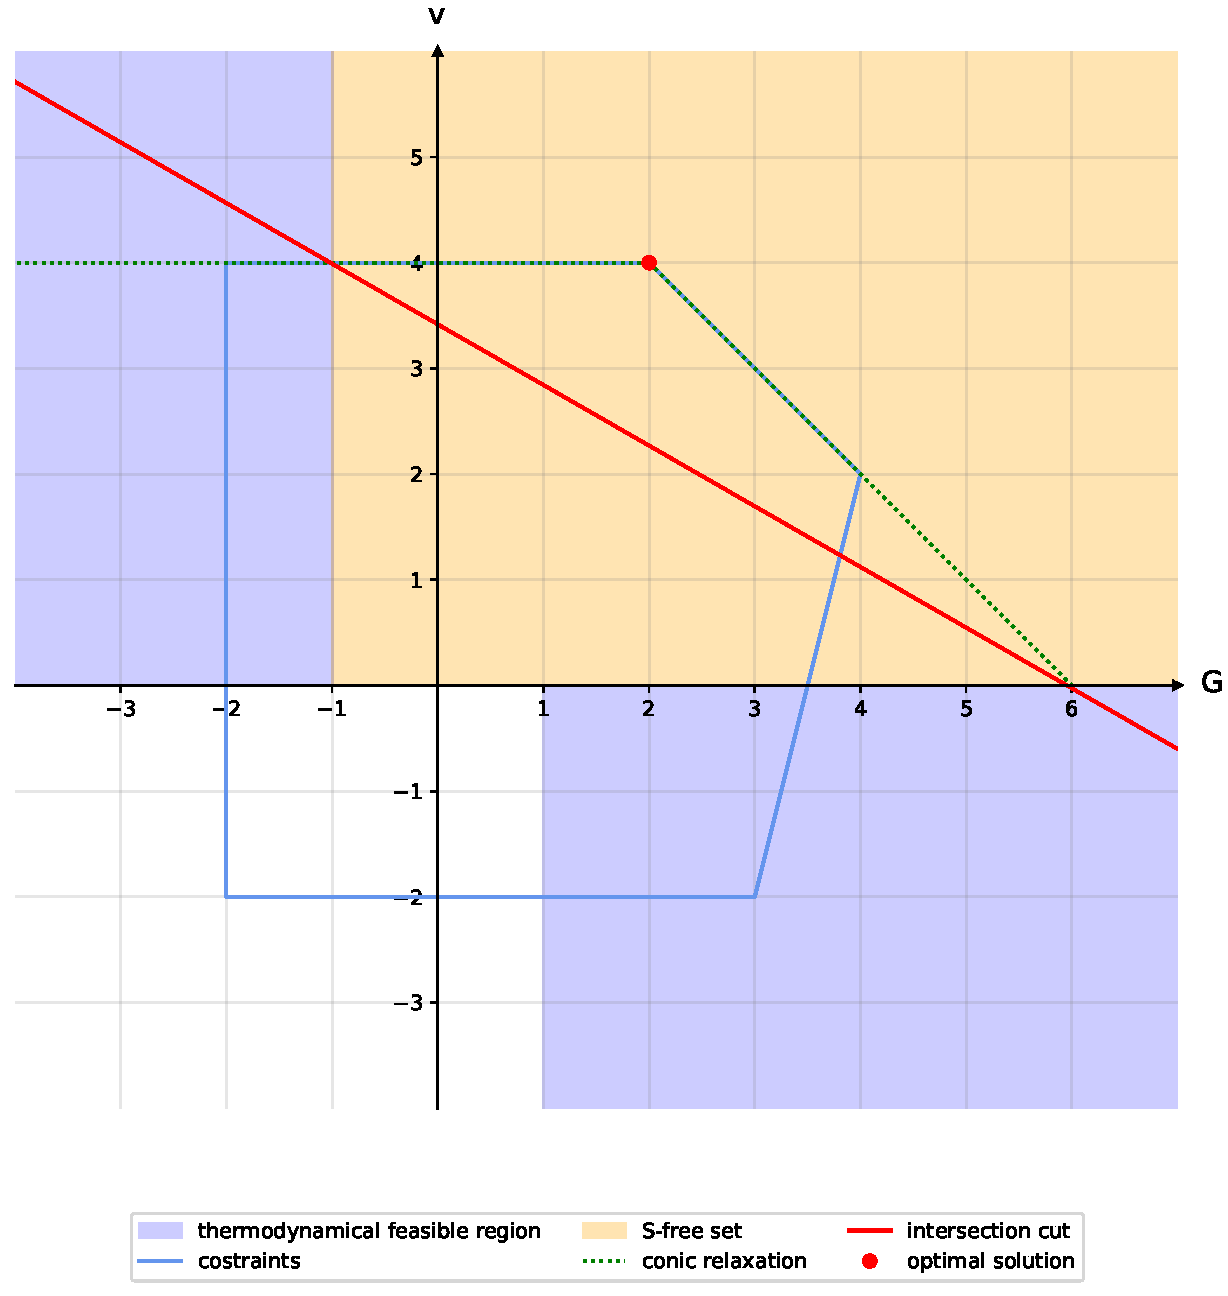
\includegraphics[width=0.8\textwidth]{Images/intersection_cut_ll_fba.pdf}
    \label{fig:intersection_cut_ll_fba}
    \subcaption*{We consider this simple model with constraints in 2D, with $\epsilon=1$. We have the decision variables $v_i, \Delta \mu_i \in \mathbb{R}$, polyhedral constraints $P$ (blue), and the set $S$ (purple area). The intersection of $S$ and $P$ is the true feasible region. Let $(\tilde{\Delta \mu}_i, \tilde v_i)$ of the optimal solution to the relaxed problem be at $(2,4)$. As $\tilde{\Delta \mu}_i$ and $\tilde v_i$ are both positive, $C_1$ is a maximal $S$-free set (yellow area). The conic relaxation at $(\tilde{\Delta \mu}_i, \tilde v_i)$ and the S-free set $C_1$ intersect at the points $(-1,4)$ and $(6,0)$. The area between the line through the intersecting points and $(\tilde{\Delta \mu}_i, \tilde v_i)$ is cut off.}
\end{figure}
% thermo_fba_bigM
\todo[inline]{make figure nice, correct labels, colour interior of polytope, fix cut off extreme ray, correct subsection}

The conic relaxation $P'$ at a relaxed solution $\boldsymbol{\tilde x}$ is a cone with apex $\boldsymbol{\tilde x}$ the extreme rays are the intersections of the active constraints. $P'$ can be written as a conic combination of extreme rays \cref{Eq:conic_relaxation} or as a polyhedron of the active constraints \cref{Eq:conic_relaxation_polyhedral}. The basic variables and nonbasic constraints defining a basis $P'$ for $\boldsymbol{\tilde x}$ can be extracted from an LP solver. 

Suppose reaction $i$ in $\boldsymbol{\tilde x}$ has $\tilde v_i >0$ and $\tilde{\Delta \mu_i} >- \epsilon$. $(\tilde v_i, \tilde{\Delta \mu_i}) \in C_1$ and $(\tilde v_i, \tilde{\Delta \mu_i}) \not \in C_2$. % and therefore $C_1$ is a maximal $S$-free set around $\tilde x$.
To compute the intersection of the conic relaxation and $C_1$, we check for each extreme ray $\bold r^j = (- \bold{\tilde A}^{-1}_{*,j})$ generated by $\tilde x$ whether it intersects the boundary of $C_1$. 
First, the intersection of the conic relaxation with the hyperplane $h_1 = \{\bold x \in \mathbb{R}^{n + m + |\mathcal{I}|} \, | \, v_i = 0 \} $ is computed. $(\boldsymbol{\tilde x} + \lambda_1 \bold r^j)_{k_1} = \bold 0$ is solved for $\lambda_1$, where $k_1$ corresponds to the index of $v_i$ in $\boldsymbol{\tilde x}$.
% Each ray $r^j$ generated by $\tilde x$ is set equal to $h_1$ and solved for $\lambda_1$: $\tilde x + \lambda_1 r^j=h_1$. 

Similarly, the intersection of each extreme ray generated by $\boldsymbol{\tilde x}$ with $h_2$ is computed, where $h_2 = \{\bold x \in \mathbb{R}^{n + m + |\mathcal{I}|} \, | \, \Delta \mu_i = -\epsilon \}$. We solve $(\boldsymbol{\tilde x} + \lambda_2 \bold r^j)_{k_2} = -\boldsymbol \epsilon$ for the step size $\lambda_2$, where $k_2$ is the index of $\Delta \mu_i$ in $\boldsymbol{\tilde x}$. 
An extreme ray intersects the boundary of $C_1$ if either $\lambda_1$ or $\lambda_2$ is finite and positive. If $\lambda_1, \lambda_2$ are both negative or if the ray does not intersect with either of the lines, there is no intersection with $C_1$ and the step size is set to $\infty$. 
\todo[inline]{explain what happens if lambda is zero or very small, or if lines are almost parallel \\ explain the geometric meaning of infinity case}

If reaction $i$ in $\tilde x$ has $v_i <0$ and $\Delta \mu_i < \epsilon$, the intersection between the conic relaxation and $C_2$ is computed analogously. The equations to solve are $(\boldsymbol{\tilde x} + \lambda_1 \bold r^j)_{k_1} = \bold 0$ and $(\boldsymbol{\tilde x} + \lambda_1 \bold r^j)_{k_2} = \boldsymbol \epsilon$.

% Suppose we have one reaction and $v, \Delta \mu \in \mathbb{R}$ which have positive values assigned. The $S$-free set $C_1$ contains the points that are greater than $s_1 = \begin{pmatrix} 1 \\ 0 \end{pmatrix} t_1$ and greater than $s_2 = \begin{pmatrix} -1 \\ 0
% \end{pmatrix} + \begin{pmatrix} 0 \\ 1 \end{pmatrix} t_2$ \todo[inline]{make vector nice}. First, the intersection of the conic relaxation with the line $s_1$ is computed. Each ray $r^j$ generated by $\tilde x$ is set equal to $s_1$ and solved for $\lambda_1$: $\tilde + \lambda_1 r^j=s_1$. Analogously, each ray generated by $\tilde x$ is set equal to $s_2$ and the step size is denoted as $\lambda_2$. The intersection with the boundary of $C_1$ is the minimum of positive $\lambda_1$ and $\lambda_2$. If $\lambda_1, \lambda_2$ are both negative or if the ray does not intersect with either of the lines, there is no intersection with $C_1$ and the step size is set to $- \infty$.
% In higher dimensions, the $S$-free set  of reaction $i$ with $v_i > 0$ and $\Delta \mu_i > -1$ is still the intersection of the two half-spaces $C_1 = \{(v, \Delta \mu) | v_i \geq 0, \, \Delta \mu_i \geq -1\}$.

% There are at least two possibilities of using intersection cuts: (1) one can either decompose the problem to solve FBA ... \todo[inline]{depends on definition of $P$} and generate cuts based on a solution to the master problem or 
% (2) one could also compute several intersection cuts from an FBA solution and add the cuts to the ll-FBA problem. 

\todo[inline]{write about possible usage of intersection cut}
\todo[inline]{write about conic relaxation extraction in detail}
\todo[inline]{example}

\subsection{Disjunctive Programming} \label{section:disjunctive_programming}
\cref{problem:llfba} written as disjunctive program is:

\begin{maxi!}
    {\scriptstyle \bold v, \boldsymbol{\Delta \mu}, \boldsymbol \mu}{\bold c^\intercal \bold v}{\label[problem]{problem:llfba_dp}}{}
    \addConstraint{\bold S \bold v= \bold 0} 
    \addConstraint{\bold l \leq \bold v \leq \bold u}
    \addConstraint{\boldsymbol{\Delta \mu}^\intercal = \boldsymbol \mu^\intercal \bold S_{\mathcal{I}}}
    \addConstraint{
        \left[\begin{array}{cc} Y_i \\ v_i \geq 0 \\ \Delta \mu_i \leq -\epsilon \end{array} \right] \lor 
        \left[\begin{array}{cc} Y_{i + |\mathcal{I}|} \\ v_i \leq 0 \\ \Delta \mu_i \geq \epsilon \end{array} \right] 
        \quad \forall i \in \mathcal{I}} \label[constraint]{constraint:llfba_dp_e}
    \addConstraint{Y_i \lor Y_{i + |\mathcal{I}|} \quad \forall i \in \mathcal{I}} \label[constraint]{constraint:llfba_dp_f}
\end{maxi!}
\quad where we have Boolean variables $Y_i \in \{true, false \}$ in addition to the continuous variables $\bold v \in \mathbb{R}^n, \boldsymbol{\Delta \mu} \in \mathbb{R}^{| (\mathcal{I})|}, \boldsymbol \mu \in \mathbb{R}^m$. %\todo[inline]{explain why you name it Boolean and not binary}

The \textsf{DisjunctiveProgramming} package extends \textsf{JuMP} and enables formulating disjunctive programs and provides several MIP reformulations \cite{perez_disjunctiveprogrammingjl_2023}
. The package is used to model \cref{problem:llfba_dp} and to acquire the big-M reformulation and the hull reformulation (see \cref{section:solving_dps}). For both reformulations the Boolean variable $Y_i$ is modeled by a binary variable $y_i$. \cref{constraint:llfba_dp_f} is then:
\begin{equation*}
    y_i + y_{i + |\mathcal{I}|} = 1 \quad \forall i \in \mathcal{I}
\end{equation*}

The big-M reformulation of \cref{constraint:llfba_dp_e} is:
\begin{align*}
    -v_i &\leq M (1 - y_i) \\
    v_i &\leq M (1- y_{i + |\mathcal{I}|}) \\
    \Delta \mu_i &\leq -\epsilon + M (1 - y_i) \\ 
    - \Delta \mu_i &\leq -\epsilon + M(1 - y_{i + |\mathcal{I}|})
\end{align*}

\quad which is identical to \cref{problem:thermo_fba_bigM} except that the big-M reformulation of \cref{problem:llfba_dp} uses two binary variables per disjunction instead of one.
The tightness of the relaxed feasible solution of the big-M reformulation depends on the scalar $M$. The package finds the optimal value of $M$ by using interval arithmetic \cite{hutchison_automating_2010}.

For the hull reformulation, two continuous variables are added for each decision variable in a disjunction. The variables corresponding to $v_i$ are denoted as $v_{i_1}$ and $v_{i_2}$ and the variables corresponding to $\Delta \mu_i$ are $\Delta \mu_{i_1}$ and $\Delta \mu_{i_2}$. The hull reformulation of \cref{constraint:llfba_dp_e} is:
\begin{align*}
    &v_i = v_{i_1} + v_{i_2} \\
    &\Delta \mu_i = \Delta \mu_{i_1} + \Delta \mu_{i_2} \\
    &v_{i_1} \leq 0 \\
    &v_{i_2} \leq 0 \\
    &\Delta \mu_{i_1} \leq - y_i \\ 
    &- \Delta \mu_{i_2} \leq -y_{i + |\mathcal{I}|} \\
    &y_i + y_{i + |\mathcal{I}|} = 1 \\
    &0 \leq v_{i_j} \leq M v_{i_j}  \quad \forall j \in \{1,2\}
\end{align*}

We see that the hull reformulation needs more decision variables and constraints than the big-M reformulation. However, the feasible region of the hull reformulation is the convex hull of the disjunctions and therefore the tightest possible convex approximation. 

% \subsection{Solvers and Packages} \label{section:solvers_packages}
% All experiments were carried out on an 8-core compute node equipped with an Intel Xeon E3-1245v5 3.50GHz CPU and 32GB RAM. We use Julia 1.7.0. The package versions used are FrankWolfe.jl v.0.2.15, Bonobo.jl v0.1.2, SCIP.jl v0.11.8

\subsection{Models} \label{section:models}
\subsubsection{BiGG}
We use a subset of metabolic networks of the \textit{biochemical, genetic, and genomic} (BiGG) database \cite{BiGG}. The models selected cover the different model sizes the smallest being \textsf{e\_coli\_core} and the largest \textsf{Recon3D}. \cref{Tab:big_model_size} lists the models including the number of metabolites and the number of reactions.

\subsubsection{Yeast}

\subsubsection{GECKO}
When adding enzyme constraints to the model, the flux rate depends on the enzymes and the flux bounds $\bold l, \bold u$ are only required to restrict the direction of a reaction.  
We use COBREXA to build the enzyme models, and we generate the enzyme data randomly.
The turnover numbers differentiate for the forward and backward direction of a reaction and therefore we split each reversible reactions into one forward and one backward reaction.
At least one enzyme is mapped to each reaction including the turnover numbers for the reaction in the forward and the turnover number for the backward direction are defined. 
%We only consider reactions involving genes, because \unsure[inline]{why?}. 
The turnover numbers are taken from a normal distribution. %10^rand(Normal(μ,1))
The protein concentrations have to be in the interval $[0, 1000]$ %\todo[inline]{gene product = protein}
. An enzyme is made up of one or more proteins.
Each protein is randomly associated with either mass group A or B, and the product mass of each group is bounded by 0.5 mml/gDW. For each protein we assign a product molar mass randomly from a Uniform distribution. 
The stoichiometric matrix including enzyme data $\bold S^{GECKO}$ has a row for each metabolite and for each protein in the nework. The columns are the metabolic reactions in addition to an enzyme balance constraint linking each isozyme to its protein compound and the reaction it catalyzes.
\todo[inline]{enzymes are protein compounds}

% gene product mass group: maps gene products to specific capacity bound IDs (each genes(model) randomly assigned to group A o B),
% gene product molar mass: molar mass of a gene product (rand(Uniform(10, 100)) for each genes(model)),
% gene product mass group bound: numeric bound of each capacity ID  (0.5 mml/gDW each)
% \unsure[inline]{genes in metabolic network?}
The size of $\bold S^{GECKO}$ is therefore much larger than $\bold S$.
As an example, the stoichiometric matrix of \textsf{e\_coli\_core} including enzyme data is of size $\mathbb{R}^{209 \times 334}$. The number of rows results from 72 metabolites and 137 proteins, and we have 334 columns, instead of 95. 
\begin{table}[!ht]
    \centering
    \begin{tabular}{lll}
    \hline
        \textbf{organism} & \textbf{\# metabolites} & \textbf{\# reactions} \\ \hline
        e\_coli\_core & 72 & 95 \\ 
        iAB\_RBC\_283 & 342 & 469 \\ 
        iIS312\_Amastigote & 606 & 519 \\ 
        iAF692 & 628 & 690 \\ 
        iSB619 & 655 & 743 \\ 
        iNF517 & 650 & 754 \\ 
        iHN637 & 698 & 785 \\ 
        iJB785 & 768 & 849 \\ 
        iNJ661 & 825 & 1025 \\ 
        iSynCJ816 & 928 & 1044 \\ 
        iJN746 & 907 & 1054 \\ 
        iJR904 & 761 & 1075 \\ 
        iEK1008 & 998 & 1226 \\ 
        iCN900 & 885 & 1229 \\ 
        iYO844 & 990 & 1250 \\ 
        iND750 & 1059 & 1266 \\ 
        iMM904 & 1226 & 1577 \\ 
        iRC1080 & 1706 & 2191 \\ 
        iAF1260 & 1668 & 2382 \\ 
        iSDY\_1059 & 1888 & 2539 \\ 
        STM\_v1\_0 & 1802 & 2545 \\ 
        iJO1366 & 1805 & 2583 \\ 
        iSbBS512\_1146 & 1910 & 2591 \\ 
        iS\_1188 & 1914 & 2619 \\ 
        iSFV\_1184 & 1917 & 2621 \\ 
        iSF\_1195 & 1917 & 2630 \\ 
        iSFxv\_1172 & 1918 & 2638 \\ 
        iML1515 & 1877 & 2712 \\ 
        iZ\_1308 & 1923 & 2721 \\ 
        iAPECO1\_1312 & 1942 & 2735 \\ 
        iECB\_1328 & 1951 & 2748 \\ 
        iETEC\_1333 & 1962 & 2756 \\ 
        iYS1720 & 2436 & 3357 \\ 
        iMM1415 & 2775 & 3726 \\ 
        RECON1 & 2766 & 3741 \\ 
        iLB1027\_lipid & 2172 & 4456 \\ 
        Recon3D & 5835 & 10600 \\ \hline
    \end{tabular}
    \caption{\label{Tab:big_model_size} Model size of used BiGG models.}
\end{table}
\unsure[inline]{organisms in textsf?}